% Unofficial University of Cambridge Poster Template
% https://github.com/andiac/gemini-cam
% a fork of https://github.com/anishathalye/gemini
% also refer to https://github.com/k4rtik/uchicago-poster

\documentclass[final]{beamer}

% ====================
% Packages
% ====================

\usepackage[T1]{fontenc}
\usepackage{lmodern}
\usepackage[orientation=portrait, size=custom,width=90,height=140,scale=1.0]{beamerposter}

\usetheme{gemini}
\usecolortheme{cuhk}
\usepackage{graphicx}
\usepackage{booktabs}
\usepackage{tikz}
\usepackage{pgfplots}
\pgfplotsset{compat=1.14}
\usepackage{anyfontsize}
\usepackage{hyperref}

% ====================
% Lengths
% ====================

% If you have N columns, choose \sepwidth and \colwidth such that
% (N+1)*\sepwidth + N*\colwidth = \paperwidth
\newlength{\sepwidth}
\newlength{\colwidth}
\setlength{\sepwidth}{0.025\paperwidth}
\setlength{\colwidth}{0.45\paperwidth}

\newcommand{\separatorcolumn}{\begin{column}{\sepwidth}\end{column}}

% ====================
% Title
% ====================

  \title{Transparent 9DTact: Tactile--Vision 3D Contact Reconstruction and Force Estimation}

  \author{Oliver Young \inst{1} \and Zhang Tao (PhD Student) \inst{1}}

  \institute[shortinst]{\inst{1} The Chinese University of Hong Kong \inst{2} University of California, Santa Cruz\\
  Supervisor: Prof. [Hongming Ren]}

  % ====================
  % Footer (optional)
  % ====================

  \footercontent{
    SURP 2025, CUHK --- 9DTact Force Estimation \hfill
    \href{mailto:ojyoung@ucsc.edu}{ojyoung@ucsc.edu}}
  % \textit{Project page: coming soon}
  % (can be left out to remove footer)


  % ====================
  % Logo (optional)
  % ====================

% helper (optional): consistent vertical centering regardless of height
\newcommand{\headerlogo}[2]{\raisebox{-0.5\height}{\includegraphics[height=#1]{#2}}}

% Left logo a bit larger, right logo a bit smaller:
\logoleft{%
  \hspace*{0.8cm}%
  \headerlogo{7.2cm}{logos/CUHK-Logo.png}% was 6.5cm
}
\logoright{%
  \headerlogo{5.8cm}{logos/UCSC-Logo.jpg}% was 6.5cm
  \hspace*{8mm}% keep right padding
}
  % \logoright{\includegraphics[height=7cm]{logos/home-institution-logo.png}}

  % ====================
  % Body
% ====================

\begin{document}

% Refer to https://github.com/k4rtik/uchicago-poster
% logo: https://www.cam.ac.uk/brand-resources/about-the-logo/logo-downloads
% \addtobeamertemplate{headline}{}
% {
%     \begin{tikzpicture}[remember picture,overlay]
%       \node [anchor=north west, inner sep=3cm] at ([xshift=-2.5cm,yshift=1.75cm]current page.north west)
%       {\includegraphics[height=7cm]{logos/unott-logo.eps}}; 
%     \end{tikzpicture}
% }

\begin{frame}[t]
\begin{columns}[t]
\separatorcolumn

\begin{column}{\colwidth}

  \begin{block}{Abstract}
  We integrate a standard camera workflow with tactile sensing in a transparent 9DTact, maintaining full RGB image/video capture while estimating contact depth and force. From frames, we create object masks using traditional OpenCV segmentation, SAM2, or their intersection. Pixel brightness/colour changes are rectified, background-removed, and mapped to depth via a calibrated Pixel$\rightarrow$Depth LUT, yielding deformation fields. We experimentally cross-reference these deformations with ground-truth forces to learn simple, interpretable mappings (mean/max/sum depth $\rightarrow$ force) and to visualize per-pixel force. The current poster emphasizes robust rectification, consistent masking, and honest evaluation: we summarize strong qualitative results and highlight challenges (mask semantics, photometric sensitivity, alignment) that inform the next iteration of calibration and benchmarking.
  \end{block}

  \begin{block}{Motivation \\ and Background}
  \begin{itemize}
    \item 9DTact is a low-cost, effective tactile sensor for shape reconstruction and force estimation with broad applications in dexterous manipulation.
    \item Aim: advance 9DTact to sense approaching objects (pre-contact awareness) while preserving accurate contact shape and force mapping after impact.
    \item Approach: combine camera-first perception (RGB, SAM2) with calibrated photometric depth to keep the system a useful camera and a tactile sensor.
    \item Focus: robust rectification, consistent mask semantics, calibrated Pixel$\rightarrow$Depth, and interpretable (simple) force models.
  \end{itemize}
  \end{block}

  \begin{block}{Hardware \& Setup}
  \begin{figure}
  \centering
  % Replace with your saved composite image path
  \includegraphics[width=.95\linewidth]{figs/hardware_overview.png}
  \caption{(a) 9D-Tact schematic highlighting the optical path and numbered parts. (b) Original 9D-Tact exploded view (numbers match labels). (c) Prototype enclosure (side) showing the transparent + translucent gel stack on an acrylic window. (d) Prototype full view with camera board and FFC.}
  \end{figure}

  \vspace{-0.5em}
  \textbf{Context (what changed)}
  \begin{itemize}
    \item \textbf{Goal:} enable on-sensor imaging/video while preserving calibrated depth sensing.
    \item \textbf{Change vs.\ legacy:} remove the opaque black gel \textbf{(12)} and LED board \textbf{(5)}; use a \textbf{transparent (10)} + \textbf{translucent (1)} silicone stack over the \textbf{acrylic window (9)}.
    \item \textbf{Housing/optics:} shell \textbf{(8)}, isolation ring \textbf{(6)}, sensor base \textbf{(2)}, camera \textbf{(4)}.
    \item \textbf{Benefit:} RGB frames for contact visualization and per-frame processing; compatible with Pixel$\rightarrow$Depth LUT pipeline.
  \end{itemize}

  \vspace{-0.25em}
  \textbf{Mini-legend (numbers $\rightarrow$ parts)}
  \begin{itemize}
    \item \textbf{1} Translucent silicone layer \hspace{1em} \textbf{2} Sensor base \hspace{1em} \textbf{4} Camera
    \item \textbf{5} (Removed) LED board \hspace{1em} \textbf{6} Isolation ring \hspace{1em} \textbf{8} Sensor shell
    \item \textbf{9} Acrylic window \hspace{1em} \textbf{10} Transparent silicone layer \hspace{1em} \textbf{12} (Removed) black gel layer
  \end{itemize}
  \end{block}

  \begin{alertblock}{Pipeline Overview}
  \textbf{1) Rectify \& Crop}: apply precomputed maps (\texttt{row\_index}, \texttt{col\_index}, \texttt{position\_scale}) and center-crop to suppress edge artifacts.\\
  \textbf{2) Contact Mask}: compute a Gaussian high-pass background removal, threshold, and morphology; optionally intersect with SAM-2 instance segments; keep the largest connected component.\\
  \textbf{3) Depth Reconstruction}: convert pixel differences to depth using a calibrated Pixel$\rightarrow$Depth LUT and a lighting threshold; smooth with small Gaussian kernels.\\
  \textbf{4) Force Features}: compute mean/max/sum depth within the contact region and record these statistics.\\
  \textbf{5) Regression \& Visualization}: fit a linear mapping from mean depth (mm) to force (N); render depth maps, point clouds, and a per-pixel force surface.
  \end{alertblock}

  % Moved/renamed section: Calibration and Camera Distortion Removal
  \begin{block}{Calibration and Camera Distortion Removal}
  Rectification aligns pixels to the gel and removes lens distortion before any masking or depth conversion. We leverage SAM2 on RGB frames to separate foreground from background when needed, while maintaining compatibility with the original 9DTact calibration flow for direct comparison. The figure shows the rectified output used to build the dataset.
  \begin{center}
    \includegraphics[width=.75\linewidth]{../9DTact/shape_reconstruction/contact_detection_results.png}
  \end{center}
  \end{block}

  \begin{block}{Contact-Region Detection}
  \textit{High-pass + threshold + morphology}: compute a Gaussian high-pass \(I_{\mathrm{hp}} = I - (G_{\sigma}\!*I)\) to remove low-frequency background, threshold to isolate deformation, and apply open/close morphology to denoise. Optionally intersect with SAM2 segments to suppress background. Key variables: \texttt{hp\_blur} (Gaussian kernel for background, larger\,$\Rightarrow$ smoother), \texttt{threshold} (binary decision on \(|I_{\mathrm{hp}}|\)), \texttt{morph\_ks} (kernel for open/close), and center-crop ratio (ROI for stability).  
  \begin{center}
    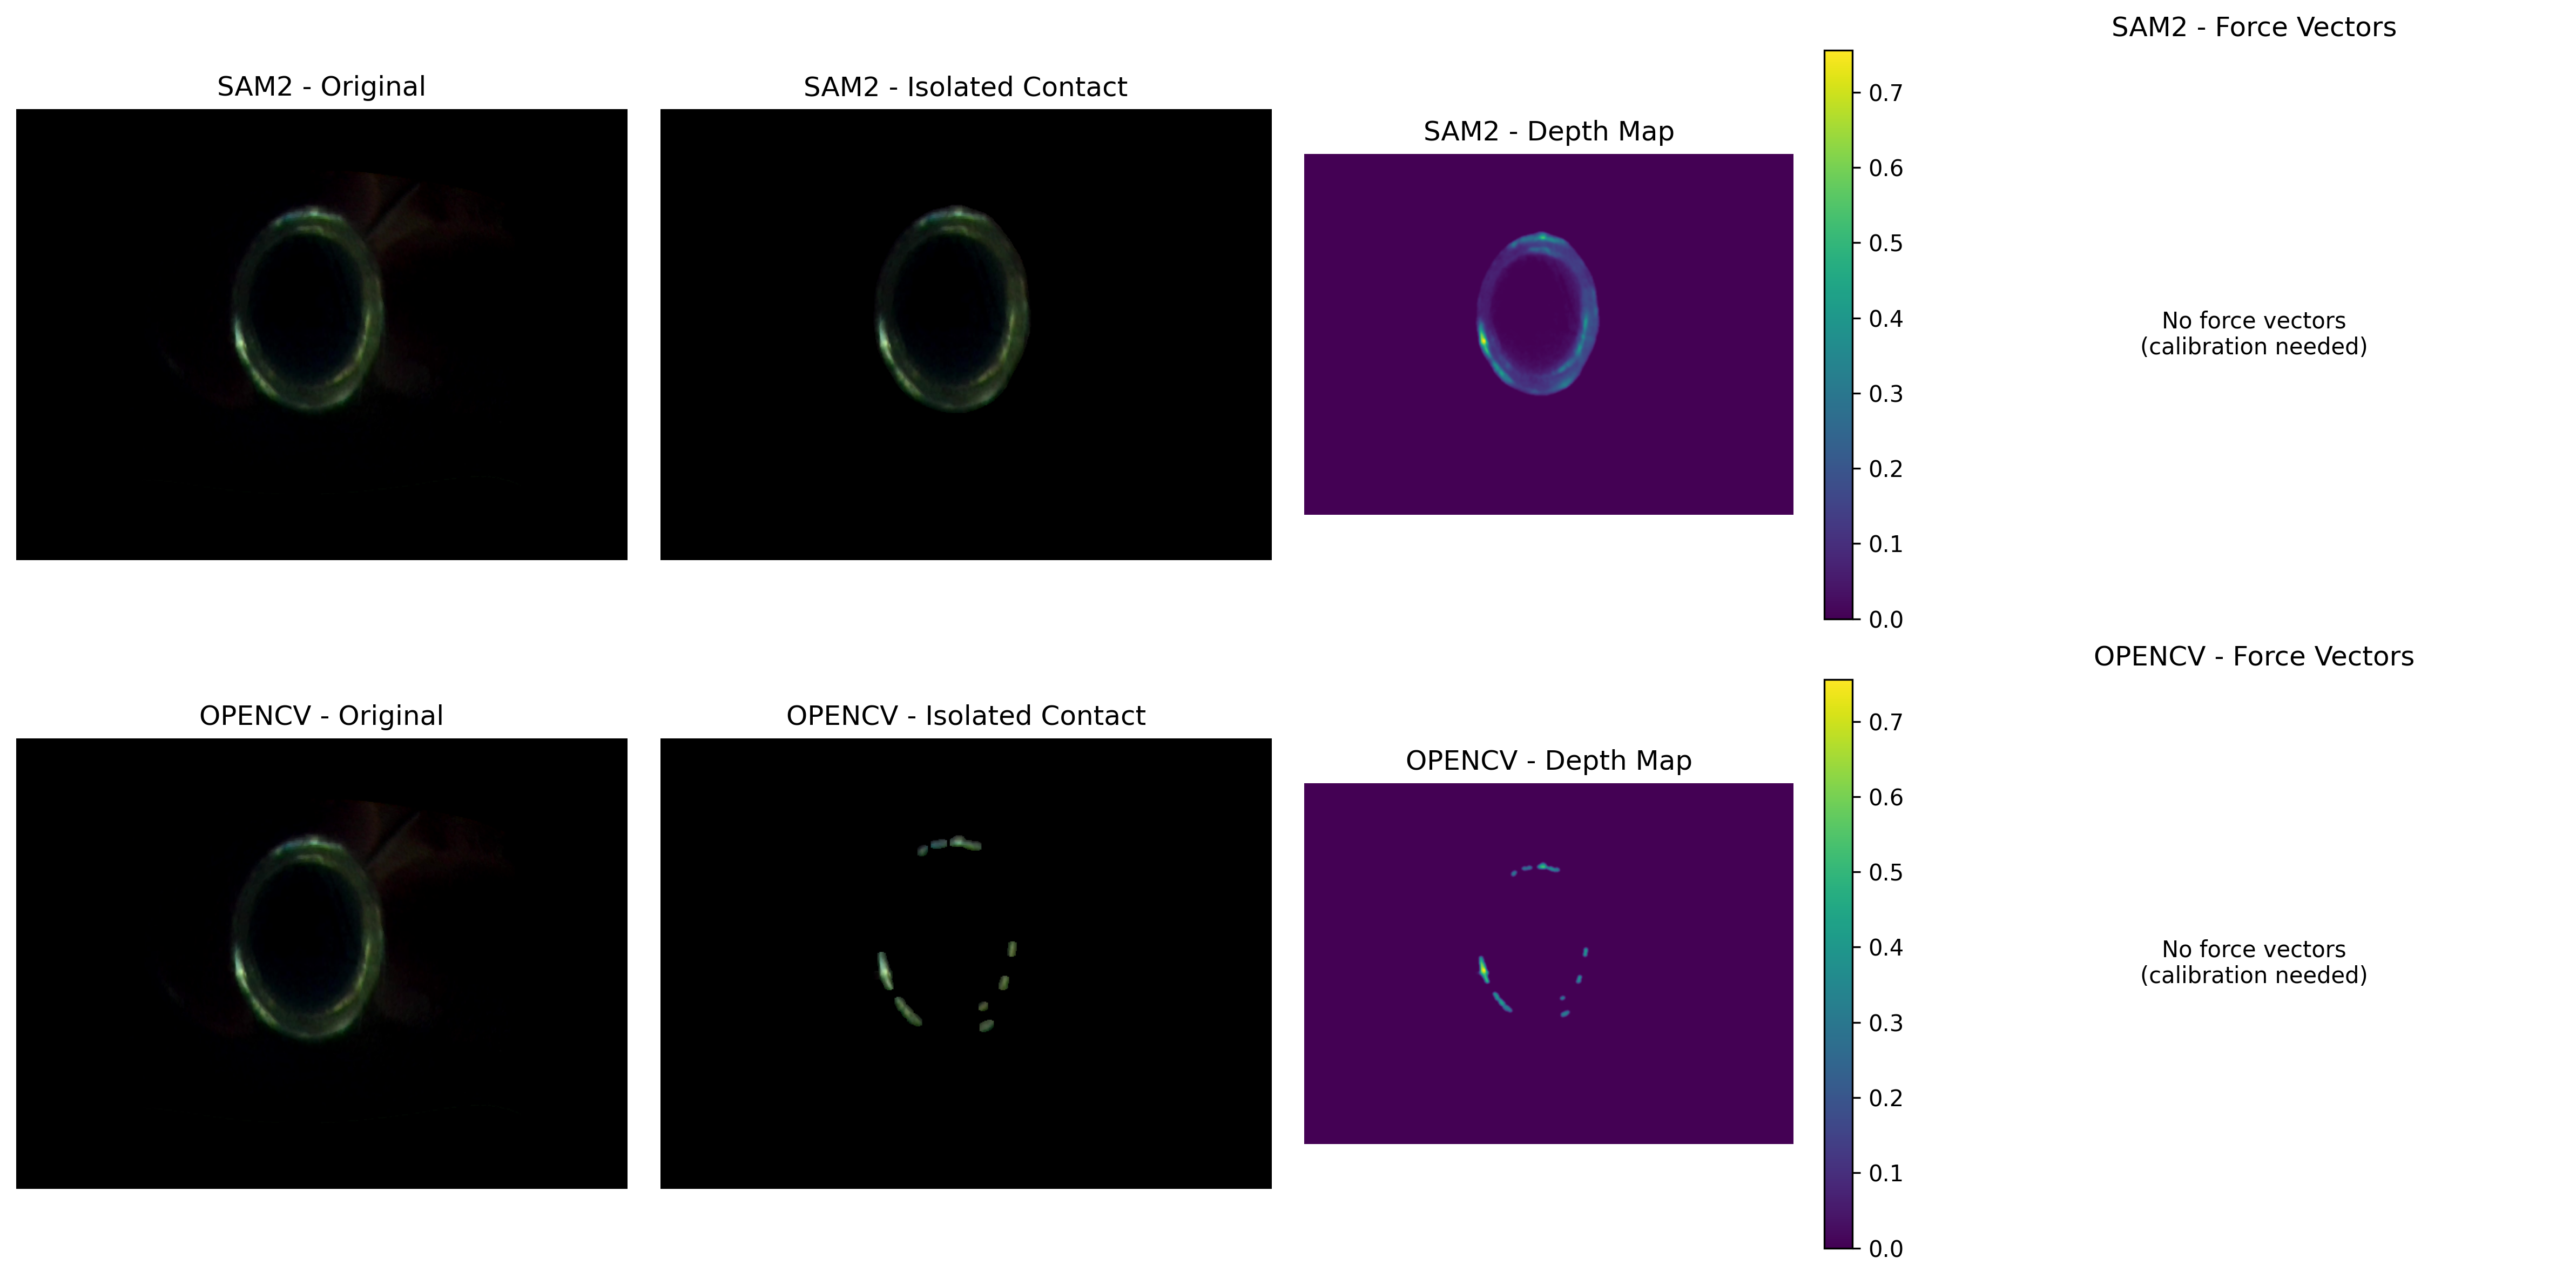
\includegraphics[width=.80\linewidth]{../9DTact/shape_reconstruction/high_sensitivity_results/comprehensive_analysis.png}
  \end{center}
  \end{block}
\end{column}

\begin{column}{\colwidth}
  % Force–deformation over time
  \begin{block}{Force--Deformation over Time}
  We map applied force against gel deformation over the acquisition sequence (negative Z; start depth 21.25\,mm). Deformation is computed as $\delta = d_{\mathrm{start}} - d_t$. The plot shows monotonic increase of $\delta$ with force and supports a first-order stiffness estimate.
  \begin{center}
    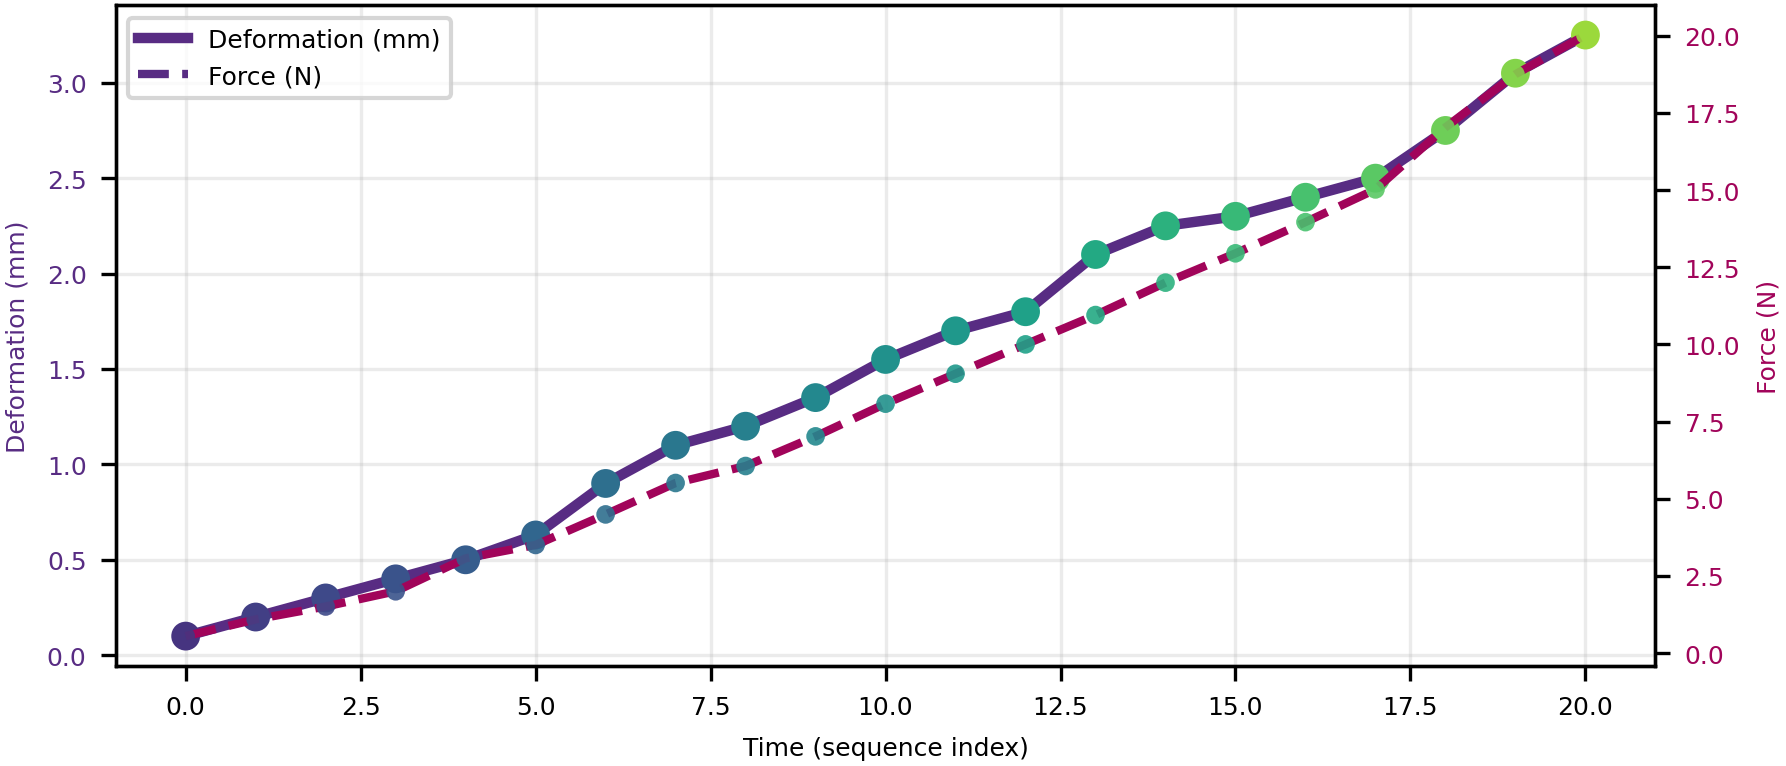
\includegraphics[width=.75\linewidth]{../9DTact/force_estimation/poster_figures/force_deformation_over_time.png}
  \end{center}
  \textbf{Rigidity (stiffness) estimate}: fit a line $F = k\,\delta + b$ over the quasi-linear region to obtain an effective stiffness $k$ (N/mm). Report $k$ with confidence intervals; check linearity (residuals) and hysteresis by sweeping up/down in force. This constant summarizes the material/system resistance to deformation under normal load and can be compared across sensors or sessions.
  \end{block}

  \begin{block}{Depth Reconstruction}
  Use a calibrated Pixel$\rightarrow$Depth LUT (\texttt{Pixel\_to\_Depth\_iterative.npy}) built from shallow-to-deep calibration video. For a pixel-difference value \(g\), depth \(d(g)\) is computed via piecewise linear mapping gated by a lighting threshold. The depth map is then smoothed with small Gaussian kernels to reduce quantization noise while preserving shape. Outputs include raw, depth, and point-cloud views.
  \begin{center}
    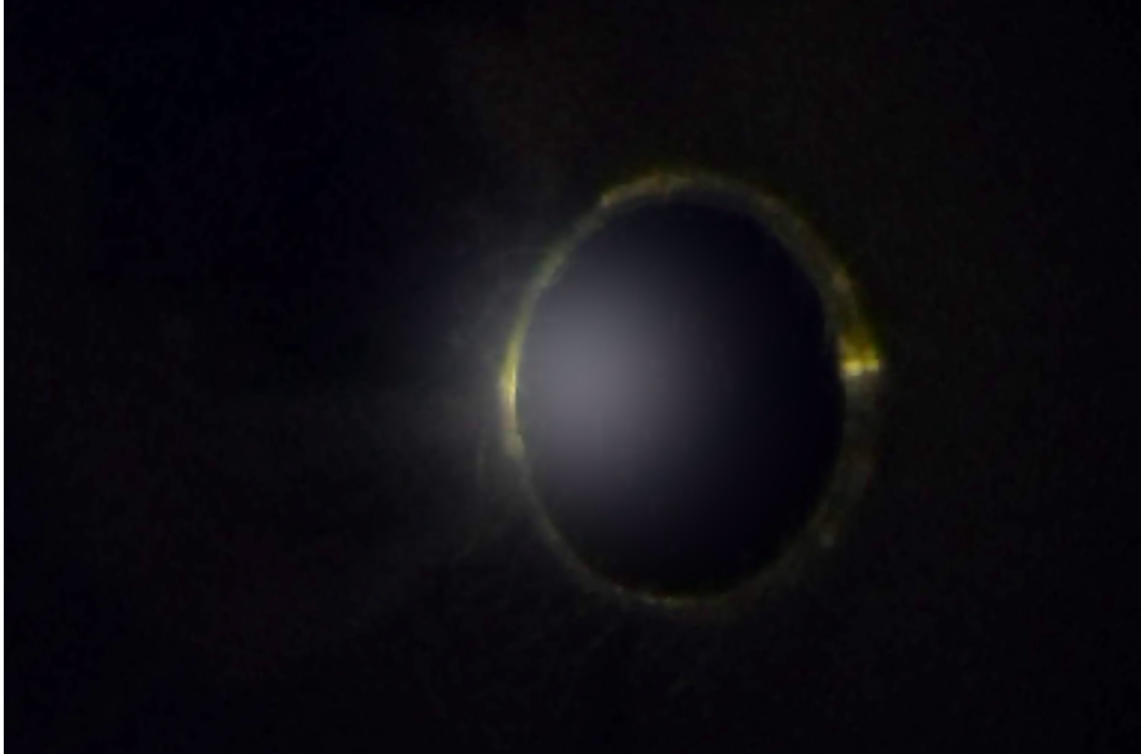
\includegraphics[width=.30\linewidth]{../9DTact/shape_reconstruction/calibration/3DModel_2/00076_raw.png}\hfill
    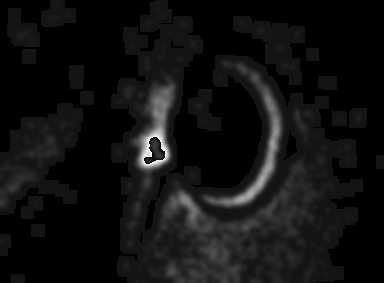
\includegraphics[width=.28\linewidth]{../9DTact/shape_reconstruction/calibration/3DModel_2/00076_depth.png}\hfill
    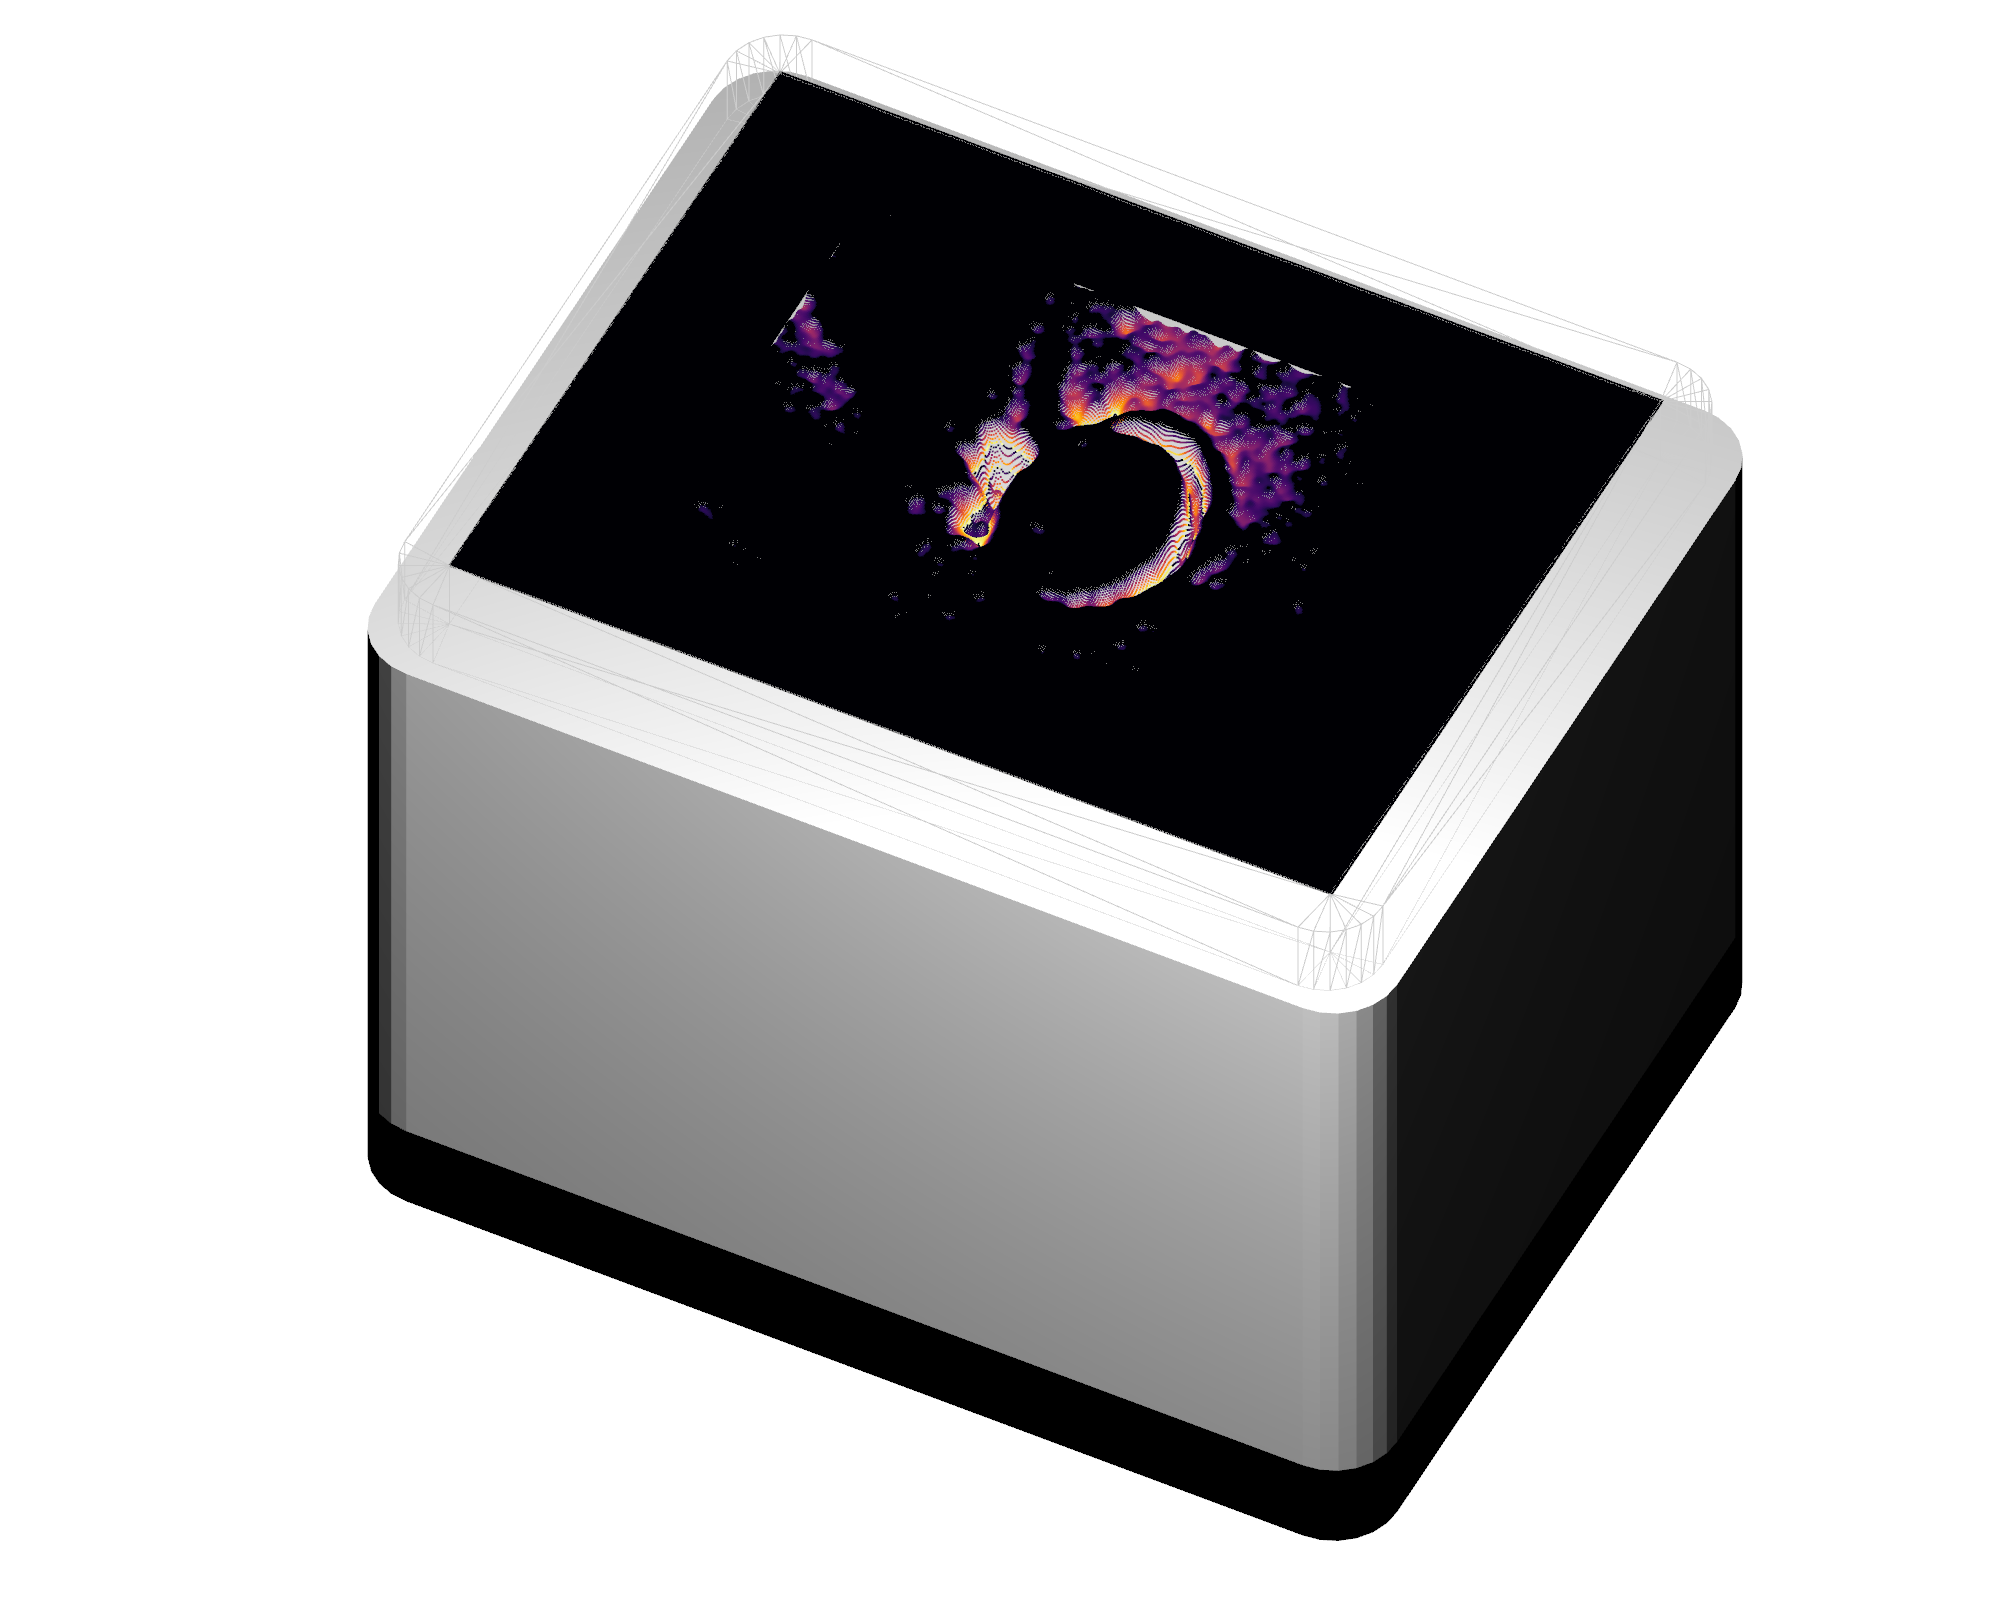
\includegraphics[width=.25\linewidth]{../9DTact/shape_reconstruction/calibration/3DModel_2/00076_pcd.png}
  \end{center}
  \end{block}

  \begin{block}{Force--Depth Dataset and Regression}
  For each labeled image (and sampled video frame), we rectify, mask the contact region, compute depth statistics (mean, max, sum), and record them to a CSV: \texttt{filename}, \texttt{force\_N}, \texttt{mean\_depth\_mm}, \texttt{max\_depth\_mm}, \texttt{sum\_depth\_mm}. A simple linear baseline predicts force as \(\hat F = \alpha\,\overline{d} + \beta\), where \(\overline{d}\) is the mean depth (mm) inside the contact mask. These features support quick parameter sweeps and baseline evaluation; non-linear mappings and learned regressors are topics for future work.
  \begin{center}
    \includegraphics[width=.47\linewidth]{../9DTact/shape_reconstruction/contact_detection_results.png}\hfill
    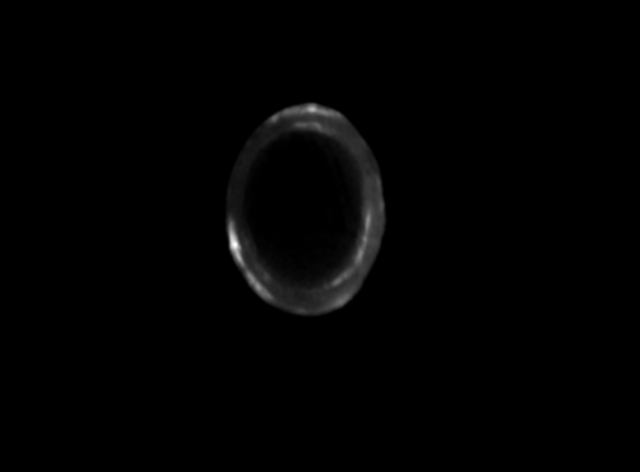
\includegraphics[width=.27\linewidth]{../9DTact/shape_reconstruction/calibration/comprehensive_analysis/sam2_depth_map.png}
  \end{center}
  \end{block}

  % --------------------
  % Case Study: 15N Example
  % --------------------
  \begin{block}{Case Study: 15N Contact and 3-D Force Visualization}
  The panels below illustrate the full pipeline on a representative 15\,N contact image. Left: contact-detection composite highlighting the segmented object and the resulting contact mask. Right: multi-panel figure showing rectified grayscale, contact-isolated view, depth map, and a 3-D force surface derived from brightness within the contact region and normalized to the labeled force.
  \begin{center}
    \includegraphics[width=.47\linewidth]{../9DTact/shape_reconstruction/calibration/comprehensive_analysis/15N_WIN_20250811_16_58_52_Pro_contact_results.png}\hfill
    \includegraphics[width=.47\linewidth]{../9DTact/force_estimation/poster_figures/15N_WIN_20250811_16_58_52_Pro_poster.png}
  \end{center}
  \vspace{0.5em}
  \textbf{Notes for interpretation:}
  \begin{itemize}
    \item \textit{Contact Mask}: high-pass filtering + threshold + morphology, intersected with SAM-2 segments to suppress background; thresholds tuned for circular objects.
    \item \textit{Depth Map}: derived via the calibrated Pixel$\rightarrow$Depth LUT; brighter hues correspond to larger indentation depths.
    \item \textit{3-D Force Surface}: per-pixel force $F(x,y)$ computed by normalizing grayscale within the mask to $[0,1]$ and scaling by the labeled force in newtons; peaks indicate higher local pressure.
  \end{itemize}
  \end{block}

  \begin{block}{Preliminary Results}
  \begin{itemize}
    \item Mean depth increases monotonically with applied force across the labeled range (\(\approx 0.5\)–\(20\)~N).
    \item Intersecting high-pass masks with SAM-2 segments yields clean, near-circular contact regions for axisymmetric indenters.
    \item 3-D force surfaces highlight pressure peaks and align with deeper basins in the depth map.
    \item Preliminary video frames show stable contact footprints and reveal transient peaks during load transitions.
  \end{itemize}
  \end{block}

  \begin{exampleblock}{Limitations and Future Work}
  \textbf{Limitations}: sensitivity to lighting, glare and haze in the transparent medium; gel aging/hysteresis; focus on normal force only; current LUTs are sensor/session-specific; cross-object generalization not yet studied.
  \vspace{0.5em}
  \textbf{Future Work}: extend to shear and torque estimation; develop temporal models (optical flow + depth) leveraging video; improve photometric calibration and SAM-2 segmentation; perform on-robot tests; explore non-linear regressors and domain adaptation across sensors and lighting conditions.
  \end{exampleblock}

  \begin{block}{Acknowledgements}
  I thank Prof. Hongliang Ren for continuous support and for providing all resources needed to make this work possible. I am especially grateful to Zhang Tao, who offered exceptional guidance throughout the program and ensured the equipment and environment were ready for experimentation. Without the mentorship of Prof. Ren and Zhang Tao, this project would not have been possible.
  \end{block}

  % References (inline)
  \begin{block}{References} 
    \footnotesize
    \begin{itemize}
      \item Luu, Q.K., Nguyen, D.Q., Nguyen, N.H., Dam, N.P., Ho, V.A. Vision-based Proximity and Tactile Sensing for Robot Arms: Design, Perception, and Control. Project website: \href{https://quan-luu.github.io/protac-website}{https://quan-luu.github.io/protac-website}.
      \item Lin, C., Zhang, H., Xu, J., Wu, L., Xu, H. 9DTact: A Compact Vision-Based Tactile Sensor for Accurate 3D Shape Reconstruction and Generalizable 6D Force Estimation. Project site: \href{https://linchangyi1.github.io/9DTact}{https://linchangyi1.github.io/9DTact}. arXiv:2308.14277.
      \item IEEE Xplore document (arnumber 11027485): \url{https://ieeexplore.ieee.org/stamp/stamp.jsp?tp=&arnumber=11027485}.
    \end{itemize}
  \end{block}

\end{column}
\separatorcolumn



\end{columns}
\end{frame}

\end{document}
